\documentclass[a4paper,12pt,reqno]{amsart}
\usepackage{graphicx}
\usepackage{macros_M53}

% pour voir les solutions il faut enlever le commentaire de la ligne suivante
% \solutionstrue

\begin{document}

% ==================================
\hautdepage{
\ifsolutions{Solutions du rattrapage}\else{Rattrapage}\fi\par\normalfont\normalsize
7 juin 2017\\{[ durée: 3 heures ]}\par
}
% ==================================
\ifsolutions\else
% {\fontencoding{U}\fontfamily{futs}\selectfont\char 66\relax}
\tikz[baseline=(e.base)]{\NoAutoSpacing\node(e){!};\draw[red,ultra thick,line join=round,yshift=-.15ex](90:1em)--(210:1em)--(330:1em)--cycle;}
\textbf{Documents autorisés :}\textit{Une feuille A4 recto-verso écrite à la main.}
\tsvp
\vspace*{\fill}
\fi


%-----------------------------------
\begin{exo} (Barycentres)

  Soient $\ens{E}$ un plan affine réel, et $\mathcal{R}= (A,B,C)$ un repère affine. On désigne par $(\alpha, \beta, \gamma)_{\mathcal{R}}$ le point dont les coordonnées barycentriques\footnote{On rappelle que $\alpha + \beta + \gamma = 1$.} sont $(\alpha, \beta, \gamma)$ dans ce repère.
  \begin{enumerate}
    \item Déterminer la nature et les paramètres de l'ensemble
      $$
        \ens{D} = \{(1,\beta,-\beta)_{\mathcal{R}} \mid \beta\in \mathbb{R}\}.
      $$
      Le représenter sur un dessin.

    \item Soit $(a,b,c) \in \mathbb{R}^{3}$ un triplet de nombres. On considère l'application
      $$
        \begin{array}[t]{lccc}
          \phi_{a,b,c} : & \ens{E}                                 & \longrightarrow & \mathbb{R} \\
                         & ( \alpha, \beta, \gamma )_{\mathcal{R}} & \longmapsto     &  a\alpha + b\beta + c\gamma
        \end{array}.
      $$
      \begin{enumerate}
        \item Montrer que $\phi_{a,b,c}$ est une application affine.
        \item Montrer que $\phi_{a,b,c}$ est constante si et seulement si $(a,b,c) \in \Delta$, où $\Delta=\{ (\lambda,\lambda,\lambda) \mid \lambda \in \mathbb{R}\}$ est la droite vectorielle \enquote{diagonale} de $\mathbb{R}^{3}$.
        \item En déduire que l'ensemble $\ens{D}_{a,b,c}=\{ (\alpha, \beta, \gamma)_{\mathcal{R}} \mid a \alpha  + b \beta  + c\gamma  = 0\}$ est une droite si et seulement si $(a,b,c) \notin \Delta$. Que peut-on dire de $\ens{D}_{a,b,c}$ dans le cas où $(a,b,c) \in \Delta$ ?
      \end{enumerate}
    \item Soient $M_1$, $M_2$ et $M_3$ trois points de $\ens{E}$. Notons $(\alpha_i,\beta_i,\gamma_i)$ les coordonnées barycentriques de $M_i$, pour $i=1,2,3$, dans le repère $\mathcal{R} = (A,B,C)$.
    \begin{enumerate}
      \item Décomposer les vecteurs $\vv{M_1M_2}$ et $\vv{M_1M_3}$ dans la base $\vv{AB}$, $\vv{AC}$ de $\ev{E}$.
      \item Montrer que $M_1$, $M_2$ et $M_3$ sont alignés si et seulement si $\begin{vsmallmatrix}\alpha_1 &\beta_1&\gamma_1\\ \alpha_2 &\beta_2&\gamma_2\\ \alpha_3 &\beta_3&\gamma_3\end{vsmallmatrix}=0$.
      \item En déduire que si $M_{1} \neq M_{2}$, la droite $\affspan{M_{1},M_{2}}$ est définie dans le repère $\mathcal{R}$ par une équation de la forme $a\alpha + b\beta + c\gamma  = 0$, avec $(a,b,c) \in \mathbb{R}^{3} \setminus \Delta$.
    \end{enumerate}
    \item Trouver un triplet $(a,b,c)$ tel que $\ens{D}_{a,b,c}$ soit la médiane du triangle $ABC$ issue de $A$.
  \end{enumerate}

\end{exo}

\begin{solution}
  \begin{enumerate}
    \item
    \begin{minipage}[t]{.70\linewidth}
      D'après la définition de $\ens{D}$, nous avons les équivalences $M \in \ens{D}$ $\Leftrightarrow$ $\exists \beta \in \mathbb{R}, M = A + \beta B - \beta C = A + \beta \vv{CB}$ $\Leftrightarrow$ $M \in A + \affspan{\vv{CB}}$. Donc $\ens{D}$ est la droite passant par $A$ de direction $\affspan{\vv{CB}}$\footnotemark.
    \end{minipage}\hspace*{\fill}\footnotetext{Le vecteurs $\vv{CB}$ est non nul car $C$ et $B$ sont des points du repère $\mathcal{R}$.}
    \begin{minipage}[t]{.28\linewidth}~\\[7mm]
      \hspace*{\fill}
      \smash{\scalebox{1.4}{\begin{tikzpicture}[etiquette/.style={scale=.35, circle, inner sep=2pt}]
	\draw
		(230:1) coordinate(A)
		(170:1) coordinate(B)
		(0:1) coordinate(C)
	;
	\draw (A) -- (B) -- (C) -- cycle;
	\draw[very thin] (A) -- +($(C)-(B)$) --+($.5*(B)-.5*(C)$) node[etiquette,above right]{$\mathcal{D}$};
	\path
		(A) node{.} node[etiquette,below]{$A$}
		(B) node{.} node[etiquette,above]{$B$}
		(C) node{.} node[etiquette,right]{$C$}
	;
\end{tikzpicture}
}}
    \end{minipage}

    \item\label{estdroite}
    \begin{enumerate}
      \item On peut directement vérifier que $\phi_{a,b,c}$ est stable par barycentre, mais on peut également observer que $\phi_{a,b,c}$ est la composée du morphisme affine $(a,b,c)_{\mathcal{R}} \mapsto (a,b,c) \in \mathbb{R}^{3}$ et de l'application linéaire $(a,b,c) \mapsto a\alpha + b\beta + c\gamma$. Donc $\phi_{a,b,c}$ est affine comme la composée de deux applications affines.
      \item Si $(a,b,c) = \lambda (1,1,1)$ alors $\phi_{a,b,c}\big((\alpha,\beta,\gamma)_{\mathcal{R}}\big) = \lambda(\alpha+\beta+\gamma) = \lambda$ est constante. Si $(a,b,c) \notin \Delta$ alors comme $a=\phi_{a,b,c}(A)$, $b=\phi_{a,b,c}(B)$ et $c=\phi_{a,b,c}(C)$ sont trois valeurs de $\im \phi_{a,b,c}$ non toutes égales, alors $\phi_{a,b,c}$ est non constante. Observons que dans ce cas comme $\im \phi_{a,b,c}$ est un sous-espace affine de $\mathbb{R}$ non réduit à un point, alors $\im \phi_{a,b,c} = \mathbb{R}$ et donc $\phi_{a,b,c}$ est surjective.
      \item Comme $\ens{D}_{a,b,c} = \phi_{a,b,c}^{-1}(0)$ il suffit d'appliquer le résultat général du cours qui nous dit que si $\ens{D}_{a,b,c}$ n'est pas vide, alors $\ens{D}_{a,b,c}$ est un espace affine de codimension égale à la codimension de $\{0\}$ dans $\im \phi_{a,b,c}$. Ainsi d'après la question précédente, si $(a,b,c) \notin \Delta$ alors $\ens{D}_{a,b,c}$ est un espace affine de codimension $1$, donc une droite, et si $(a,b,c) \in \Delta$ alors $D_{a,b,c}$ est tout $\ens{E}$ ou vide en fonction de si $(a,b,c)=(0,0,0)$ ou si $(a,b,c)=(\lambda,\lambda,\lambda)$ avec $\lambda \neq 0$.
    \end{enumerate}
    \item
    \begin{enumerate}
      \item Comme $M_{i} = (1- \beta_{i} - \gamma_{i})A + \beta_{i} B + \gamma_{i} C$, alors $\vv{AM_{i}} =  \beta_{i} \vv{AB} + \gamma_{i} \vv{AC}$ et donc par la relation de Chasles $\vv{M_{1}M_{2}} = (\beta_{2} - \beta_{1}) \vv{AB} + (\gamma_{2} - \gamma_{1}) \vv{AC}$ et $\vv{M_{1}M_{3}} = (\beta_{3} - \beta_{1}) \vv{AB} + (\gamma_{3} - \gamma_{1}) \vv{AC}$.
      \item Les trois points $M_1$, $M_2$ et $M_3$ sont alignés si et seulement si les deux vecteurs $\vv{M_{1}M_{2}}$ et $\vv{M_{1}M_{3}}$ sont colinéaires, et donc d'après la question précédente si et seulement si
      $$
        \begin{vmatrix}
          \beta_{2} - \beta_{1} & \gamma_{2} - \gamma_{1}\\
          \beta_{3} - \beta_{1} & \gamma_{3} - \gamma_{1}
        \end{vmatrix} = 0.
      $$
      Pour conclure il suffit de démontrer que ce déterminant est égal à celui de l'énoncé.
      Par des opérations sur les colonnes, en utilisant que $\alpha_{i} + \beta_{i} + \gamma_{i} = 1$, et des opérations sur les lignes, on trouve que
      $$
        \begin{vmatrix}
          \alpha_1 & \beta_1 & \gamma_1 \\
          \alpha_2 & \beta_2 & \gamma_2 \\
          \alpha_3 & \beta_3 & \gamma_3
        \end{vmatrix}
        =
        \begin{vmatrix}
          1 & \beta_1 & \gamma_1 \\
          1 & \beta_2 & \gamma_2 \\
          1 & \beta_3 & \gamma_3
        \end{vmatrix}
        =
        \begin{vmatrix}
          1 & \beta_1               & \gamma_1                \\
          0 & \beta_{2} - \beta_{1} & \gamma_{2} - \gamma_{1} \\
          0 & \beta_{3} - \beta_{1} & \gamma_{3} - \gamma_{1}
        \end{vmatrix}
        =
        \begin{vmatrix}
          \beta_{2} - \beta_{1} & \gamma_{2} - \gamma_{1}\\
          \beta_{3} - \beta_{1} & \gamma_{3} - \gamma_{1}
        \end{vmatrix}.
      $$
      \item Si $M_{1} \neq M_{2}$ alors $M \in \affspan{M_{1},M_{2}}$ si et seulement si $M_1$, $M_2$ et $M$ sont alignés. D'après la question précédente, ceci est équivalent à
      $
       \begin{vsmallmatrix}
          \alpha_1 & \beta_1 & \gamma_1 \\
          \alpha_2 & \beta_2 & \gamma_2 \\
          \alpha   & \beta   & \gamma
        \end{vsmallmatrix}
        =0
      $,
      où $(\alpha,\beta,\gamma)_{\mathcal{R}} = M$. En développant le déterminant selon la dernière ligne de la matrice, on trouve que cette équation s'écrit sous la forme $a\alpha + b\beta + c\gamma  = 0$ avec
      $
        a = \begin{vsmallmatrix}
              \beta_{1} & \gamma_{1} \\
              \beta_{2} & \gamma_{2}
            \end{vsmallmatrix}
      $,
      $
        b = - \begin{vsmallmatrix}
                \alpha_{1} & \gamma_{1} \\
                \alpha_{2} & \gamma_{2}
              \end{vsmallmatrix}
      $ et
      $
        c = \begin{vsmallmatrix}
              \alpha_{1} & \beta_{1} \\
              \alpha_{2} & \beta_{2}
            \end{vsmallmatrix}
      $.
      Pour conclure $(a,b,c) \notin \Delta$ car sinon $\affspan{M_{1},M_{2}}$ ne serait pas une droite, d'après la question \ref{estdroite}).
    \end{enumerate}
    \item La médiane sortant de $A$ est la droite engendrée par $A=(1,0,0)_{\mathcal{R}}$ et le milieu $\frac{1}{2}(B+C)=(0,\frac{1}{2},\frac{1}{2})_{\mathcal{R}}$ de $\convhull{BC}$. Ainsi d'après la question précédente, on trouve que l'équation de cette droite est $\{ -\frac{1}{2}\beta + \frac{1}{2}\gamma = 0\}$ $\Leftrightarrow$ $\{ \beta - \gamma = 0\}$.
  \end{enumerate}
\end{solution}

%-----------------------------------
\begin{exo} (Géométrie du plan complexe)

  \begin{minipage}[t]{.70\linewidth}
    Soit $ABCD$ le rectangle du plan complexe dont les sommets $A$,$B$ et $D$ ont pour affixes respectives $0$,$1$ et $i$. On considère le triangle équilatéral $BFC$ construit à l'extérieur du rectangle $ABCD$, ainsi que le triangle équilatéral $DEC$ construit à l'intérieur du rectangle $ABCD$.
  \end{minipage}
  \begin{minipage}[t]{.21\linewidth}~\\[17mm]
    \hspace*{\fill}
    \smash{\scalebox{2}{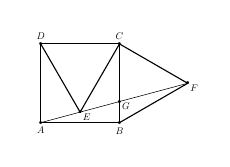
\begin{tikzpicture}[etiquette/.style={scale=.35, circle, inner sep=2pt}]
	%\draw[help lines] (-1,-1) grid (3,3);
	\draw (0,0) rectangle (1,1);
	\draw (0,1) -- +(-60:1) coordinate (E) -- (1,1);
	\draw (1,0) -- +(30:1)  coordinate (F) -- (1,1);
	\draw[very thin] (0,0) -- (F);
	\coordinate (G) at (1,{2-sqrt(3)});
	\path
		(0,0) node{.} node[etiquette,below]{$A$}
		(1,0) node{.} node[etiquette,below]{$B$}
		(1,1) node{.} node[etiquette,above]{$C$}
		(0,1) node{.} node[etiquette,above]{$D$}
		(E) node{.} node[etiquette,anchor=145]{$E$}
		(F) node{.} node[etiquette,anchor=145]{$F$}
		(G) node{.} node[etiquette,anchor=145]{$G$}
	;
\end{tikzpicture}}}
  \end{minipage}

  \begin{enumerate}
    \item Déterminer les affixes des points $E$ et $F$.
    \item Montrer que $A$, $E$ et $F$ sont alignés.
    \item Déterminer l'affixe du point $G$ qui est l'intersection des segments $\convhull{BC}$ et $\convhull{EF}$.
    \item Donner l'expression analytique de l'homothétie de centre $G$ qui envoie $A$ sur $F$.
  \end{enumerate}


\end{exo}

\begin{solution}
  \begin{enumerate}
    \item Comme $E$ est obtenu à partir de $C$ par rotation de $-\frac{\pi}{3}$ autour de $D$, nous avons $E = D+R_{-\frac{\pi}{3}}(\vv{DC})$ et donc l'affixe de $E$ est $z_{E} = i+e^{-\frac{\pi}{3}}1 = \frac{1}{2} + \frac{2-\sqrt{3}}{2} i$. Et comme $F = B + R_{-\frac{\pi}{3}}(\vv{BC})$ l'affixe de $F$ est $z_{F} = 1 + e^{-\frac{\pi}{3}}i = \frac{2+\sqrt{3}}{2} + \frac{1}{2}i$.
    \item Comme $(2+\sqrt{3})\left(\frac{1}{2} + \frac{2-\sqrt{3}}{2} i\right) = \frac{2+\sqrt{3}}{2} + \frac{1}{2}i$ nous observons que l'affixe de $\vv{AF}$ (qui est la même que celle de $F$ car l'affixe de $A$ est $0$) est un multiple réel $(2+\sqrt{3})$ de l'affixe de $\vv{AE}$ (identique à celle de $E$). Et donc les deux vecteurs sont colinéaires, et par conséquent les trois points $A$, $E$ et $F$ sont alignés.
    \item La partie réelle de l'affixe de $G$ est $1$ (car identique à celle de $B$). Et comme les trois points $A$, $E$ et $G$ sont alignés, l'affixe de $G$ est un multiple réel de l'affixe de $E$ (dont la partie réelle est $\frac{1}{2}$). En comparant les parties réelles, on constate que le multiplicateur est $2$ et donc que l'affixe recherchée de $G$ est $z_{G} = 2 z_{E} = 1+(2-\sqrt{3}) i$.
    \item L'expression analytique d'une homothétie de centre $z_{G}$ est de la forme $z \mapsto z_{G} + \lambda (z-z_{G})$. Donc il suffit qu'on détermine le réel $\lambda$, et pour cela il suffit de savoir que l'image de l'affixe $0$ de $A$ est $z_{F}$. Ainsi $\lambda = \frac{z_{G}-z_{F}}{z_{G}} = \frac{2z_{E}-(2+\sqrt{3})z_{E}}{2z_{E}} = -\frac{\sqrt{3}}{2}$ et donc l'expression analytique est $ z \mapsto -\frac{\sqrt{3}}{2}z + \frac{2+\sqrt{3}}{2} + \frac{1}{2}i $.
  \end{enumerate}
\end{solution}

%-----------------------------------
\begin{exo} (Isométries dans $\mathbb{R}^{3}$)

  On se place dans l'espace affine euclidien $\mathbb{R}^{3}$.

  \begin{enumerate}
    \item On considère les deux matrices
    \[
      \renewcommand{\arraystretch}{.77}
      \frac{1}{9}
      \begin{pmatrix*}[r]
        -1 & -8 &  4 \\
        -8 & -1 & -4 \\
         4 & -4 & -7
      \end{pmatrix*}
      \qquad\text{et}\qquad
      \frac{2}{9}
      \begin{pmatrix*}[r]
        -1 & -8 &  4 \\
        -8 & -1 & -4 \\
         4 & -4 & -7
      \end{pmatrix*}
    .\]
    Laquelle de ces deux matrices est la matrice d'une isométrie de $\mathbb{R}^{3}$ ?
  \end{enumerate}

  \emph{Pour la suite de l'exercice, on note $M$ cette matrice de $O(\mathbb{R}^{3})$, ainsi que l'application linéaire qu'elle définit.}

  \begin{enumerate}[resume]

    \item Décrire $M$ en détail (nature, paramètres).

    \item Soit $T_{\vv{v}}$ la translation de vecteur $\vv{v} = (1,1,0)$. Quelle est la nature de l'application composée $T_{\vv{v}}M$ ?

    \item Soit $S$ la symétrie orthogonale par rapport au plan d'équation $\{2x-2y+z=1\}$. Quels sont la nature et les paramètres de l'application composée $MS$ ?
  \end{enumerate}
\end{exo}

\begin{solution}
  % walfram alpha : {{-1,-8,4},{-8,-1,-4},{4,-4,-7}}/9
  % octave : M = [-1 -8 4 ; -8 -1 -4 ; 4 -4 -7]/9

  % Les espaces propres de $M$ sont $E_{1}=\affspan{(2,-2,1)}$ et $E_{-1}=\affspan{(1,1,0),(1,0,-2)}$.
  % Le polynomé charactéristique est $x^{3}+x^{2}-x-1$.

  \begin{enumerate}
    \item Les vecteurs colonnes des deux matrices forment une base orthogonale, mais seulement ceux de la première forment une b.o.n. (ceux de la deuxième sont de norme $2$). Donc la matrice orthogonale $M$ est la première matrice\footnote{On peut vérifier par exemple que $M^{t}M=\id$.}.
    \item Comme $\det(M)=1$, $M$ est une rotation. Pour trouver l'axe de rotation on cherche l'ensemble des vecteurs fixes : $\ker(M-I)$, et on trouve $E_{1}=\affspan{(2,-2,1)}$. Soit $\theta$ l'angle de rotation. Comme $2\cos(\theta)+1=\tr(M)=-1$ on trouve que $\theta=\pi$. Ainsi $M$ est une rotation d'angle $\pi$ autour de l'axe $\affspan{(2,-2,1)}$, autrement dit c'est une symétrie\footnote{Comme $M$ est symétrique on aurait pu conclure directement que $M$ est une symétrie.} axiale d'axe $\affspan{(2,-2,1)}$.
    \item Comme $\vv{v} \perp (2,-2,1)$, d'après le cours, $T_{\vv{v}}M$ est aussi une symétrie axiale.
    \item Comme le plan $\{2x - 2y + z = 1\}$ est perpendiculaire à $\affspan{(2,-2,1)}$, la composé $MS$ est une symétrie centrale de centre $\{2x - 2y + z = 1\} \cap \affspan{(2,-2,1)} = {(\frac{2}{9},-\frac{2}{9},\frac{1}{9})}$. En réalité dans une base orthonormée $(\vv{e}_{1}, \vv{e}_{2}, \vv{e}_{3})$ avec $\vv{e}_{1}=\frac{1}{3}(2,-2,1)$ nous avons les parties linéaires qui sont $\vv{M}=\begin{psmallmatrix}1&0&0\\0&-1&0\\0&0&-1\end{psmallmatrix}$, $\vv{S}=\begin{psmallmatrix}-1&0&0\\0&1&0\\0&0&1\end{psmallmatrix}$, et donc $\vv{MS}=-\id$.
  \end{enumerate}
\end{solution}



%-----------------------------------
\begin{exo} (Coniques)

On considère l'ensemble
  \[
    \ens{E}=\{ (x,y) \in \mathbb{R}^{2} \mid (x+y-1)^{2}+2(x-y)^{2}=4\}.
  \]

  \begin{enumerate}
    \item Montrer que $\ens{E}$ est une ellipse.
    \item Déterminer les coordonnées du centre de $\ens{E}$, ainsi que les rayons.
    \item Déterminer les axes de symétrie de $\ens{E}$ et donner les expressions analytiques des symétries par rapport à ces axes.
    \item Déterminer les coordonnées des foyers de $\ens{E}$.
  \end{enumerate}

\end{exo}

\begin{solution}
  \begin{enumerate}
    \item On pose $X = \frac{x+y-1}{\sqrt{2}}$ et $Y = \frac{x-y}{\sqrt{2}}$. Comme la partie linéaire
      $ \frac{1}{\sqrt{2}}
        \begin{psmallmatrix*}[r]
          1 & 1 \\
          1 & -1
        \end{psmallmatrix*}
      $ de ce changement de variables est orthogonale, alors l'équation de $\ens{E}$ dans la nouveau repère orthonormé $\mathcal{R}'$ est $ \frac{X^{2}}{2}+\frac{Y^{2}}{1}=1$. Ainsi d'après le cours, $\ens{E}$ est une ellipse de rayons $R = \sqrt{2}$ et $r = 1$.
    \item Les rayons ont été déjà déterminés dans la question précédente. Le centre de l'ellipse a pour coordonnées $X=0$ et $Y=0$ dans le nouveau repère $\mathcal{R}'$, donc il s'agit du point de coordonnées $(x_{0},y_{0}) = (\frac{1}{2}, \frac{1}{2})$.
    \item Les axes de symétrie ont pour équations dans la nouvelle base $X=0$ et $Y=0$, donc il s'agit des droites d'équations $x+y-1=0$ et $x-y=0$. Les expressions analytiques dans la nouvelle base des deux symétries sont respectivement $(X,Y)_{\mathcal{R}'} \mapsto (-X,Y)_{\mathcal{R}'}$ et $(X,Y)_{\mathcal{R}'} \mapsto (X,-Y)_{\mathcal{R}'}$. Ainsi la symétrie par rapport à la droite $\{x+y-1\}$ est $(x,y) = \frac{1}{\sqrt{2}}(x+y-1,x-y)_{\mathcal{R}'} \mapsto \frac{1}{\sqrt{2}}(1-x-y,x-y)_{\mathcal{R}'} = (1-y,1-x)$. De même, on trouve que la symétrie par rapport à la droite $\{x-y=0\}$ est $(x,y) \mapsto (y,x)$.
    \item Les foyers se trouvent sur le grand axe $\{x-y=0\}$ à distance $\sqrt{R^{2}-r^{2}} = 1$ du centre $(\frac{1}{2}, \frac{1}{2})$. Comme un vecteur directeur du grand axe est $(\frac{1}{\sqrt{2}},\frac{1}{\sqrt{2}})$, nous pouvons conclure que les coordonnées des deux foyers sont
    $$
      (\frac{1}{2}, \frac{1}{2}) \pm (\frac{1}{\sqrt{2}},\frac{1}{\sqrt{2}}) = (\frac{1}{2} \pm \frac{1}{\sqrt{2}}, \frac{1}{2} \pm \frac{1}{\sqrt{2}}).
    $$
  \end{enumerate}

\end{solution}


\end{document}
